\section{Introduction}
Since the microelectronics revolution, Silicon has been a dominant material 
for the production of devices for a variety of applications. Silicon has 
non-ideal properties for a variety of applications but remains dominant due 
to its well-understood processing parameters and large manufacture install 
base, providing economies of scale. The III-V semiconductors offer superior 
properties for a variety of applications when compared to silicon, and are 
actively used in applications were performance is valued above other 
considerations, such as military and space sectors. The goal of integrating 
III-V semiconductors into silicon based microelectronics has spawned extensive 
research into the processing involved to grow or otherwise electronically 
attach these materials with minimal defects.

Under auspices of the ARISE Photovoltaics project, the III-V 
semiconductors GaAs, GaSb, AlSb and InP were grown as thin films under a 
variety of conditions on single crystal silicon substrates, in order to 
examine the growth process and electro-optic properties. The role of the 
varied lattice mismatch, growth parameters, and substrate properties were 
examined and several previously undocumented phenomona were examined due to 
the use of 2DXRD, whose benefits were documented in \cref{sec:2DXRD}.

The formation of epitaxial (or growth) twins was found to be a key area where 
the literature had performed little examination. The role of twins in the 
formation of electronic defect networks, and the effects vicinal (offcut) 
substrates had on their formation were thoroughly examined and a 
explanatory model was developed to explain factors that affect their formation 
and provide proposed routes towards their minimization and 
elimination\cite{Devenyi2011}. This work was completed in close collaboration 
with Ms. Steffi Woo, a Ph.D. candidate in Material Science and Engineering and 
McMaster, with the TEM/STEM work performed exclusively by her and all other 
work being collaborative.

\section{Background}
\todo{Should a section covering the background of III-V on Silicon go here, or 
go into the introductory material at the beginning of the thesis}

\section{Experimental} \todo{This section is currently copy-pased from 
paper, is this appropriate?}
Semiconductor thin films (GaAs, InP, GaSb, and AlSb) were deposited on nominal 
(001)-oriented (\(\pm\)0.5\(^\circ\)) and vicinal Si substrates (offcut 
4.7\(^\circ\) (\(\pm\)0.25\(^\circ\)) towards [110]) using a SVT Associates 
molecular beam epitaxy (MBE) system. As-received epi-ready wafers were cleaned 
for 1 min in a 4\% HF in deionized (DI) water dip followed by a 30 sec DI 
rinse immediately prior to their insertion into the MBE load-lock. Before film 
deposition, both the nominal and vicinal Si(001) substrates underwent a 15 min 
degassing procedure at 350~\(^\circ\)C followed by a thermal treatment at 
800~\(^\circ\)C for up to 5 min, in order to reconstruct the Si surface into 
single domain 
terraces\cite{NeergaardWaltenburg1995,S1991,Sakamoto1986,Pehlke1991}. A small 
number of single steps are expected to remain on vicinal substrates, a higher 
number on nominal substrates because of the larger terrace length. Growth 
conditions followed established 
protocols\cite{Akahane2004,Balakrishnan2006a,Fischer1986} and yielded 
comparable rocking curve full-width half-maximum for the [004] reflection 
using double crystal X-ray diffraction. AlSb thin films were grown to a 
thickness of 550~nm with a 20~nm GaSb capping layer to avoid oxidation. GaAs 
thin films was grown to a thickness of 600~nm and GaSb to a thickness of 
500~nm. InP samples were grown at 470~\(^\circ\)C with a V/III flux ratio of 2 
at a growth rate of 1 \(\mu m\)/hr, resulting in a thickness of 600~nm. Double 
crystal X-ray and TEM data also revealed that all films are fully relaxed by a 
network of interracial misfit dislocations\cite{Vajargah2011}. GaSb samples 
were grown in the presence of a 5 nm AlSb buffer layer, as prescribed by 
Akahane \textit{et al}.\cite{Akahane2004}.

Stereographic pole figures were generated for each sample using 2DXRD 
techniques. A Bruker SMART 6000 CCD detector on a Bruker 3-circle D8 
goniometer (Bruker AXS Inc., Madison, WI) with a Rigaku RU-200 rotating anode 
X-ray generator (Rigaku MSc, The Woodlands, TX) and parallel-focusing 
monochromator optics was used for the data collection. Scans were taken with 
the detector centered on the (111) 2\(\theta\) of the material of interest and 
the sample rotated through 360\(^\circ\) in 0.5\(^\circ\) increments about the 
surface normal of the sample. A 1D integration of all frames was used to 
determine the combined width of the (111) peaks using MAX3D software (McMaster 
University)\cite{Britten2007}. The peak width was then used to integrate (111) 
reflections from all frames, including a background and absorption correction 
for the corresponding material with GADDS (Bruker-AXS) software, resulting in 
a pole figure. Pole intensities were obtained from pole figures using a 
circular integration cursor with a 10 pixel radius which was centered on the 
pole so as to maximize the total intensity captured. All pole intensities were 
corrected for structure factor and frame exposure times.

For each sample two \{110\} TEM cross-sections were prepared, one parallel to 
the [110] miscut direction and the other perpendicular. The specimens were 
prepared by the standard procedure of mechanical polishing, dimpling, and 
ion-milling (4 keV Ar-ions at an incident angle of \(\pm\)4\(^\circ\) using a 
liquid nitrogen cold stage for InP) until perforation. Crystallographic 
information of the epitaxial layer was obtained using diffraction contrast 
imaging with a Philips CM12 conventional transmission electron microscope 
(TEM) operated at 120 kV and equipped with a LaB\(_6\) filament. In addition, 
electron diffraction analysis was performed using selected area electron 
diffraction (SAD).
\section{Results}
2DXRD measurements performed on as-grown thin films indicated a bulk 
orientation of the material consistent with epitaxial alignment with the 
single crystal silicon substrate. The pole figures generated from 2DXRD data, 
such as \cref{fig:twins_pole_example} also contained a number of other peaks 
at reduced intensity indicating other orientations of the material of interest 
other than the bulk orientation. In order to develop a comprehensive picture 
of the distribution of the grown thin films, simulated pole figures were 
examined in an attempt to generate a composite pole figure which qualitatively 
matched the figures generated from data. Based on these simulations, the 
simulated pole figure \cref{fig:twins_sim_polefigure} was developed, 
indicating that the thin films consisted of a bulk epitaxial phase, and four 
primary twin phases, along with secondary twin phases (not shown). The primary twins form 
along (111), (1\(\overline{1}\)1) (\(\overline{1}\overline{1}\)1) and (\(\overline{1}\)11) 
habit planes.
\begin{figure}
    \begin{subfigure}[b]{0.5\linewidth}
        \centering
        \missingfigure{Representative Single Pole Figure}
        \caption{A representative pole figure of GaAs grown on nominal (100) 
        Silicon\label{fig:twins_pole_example}}
    \end{subfigure}
    \begin{subfigure}[b]{0.5\linewidth}
        \centering
        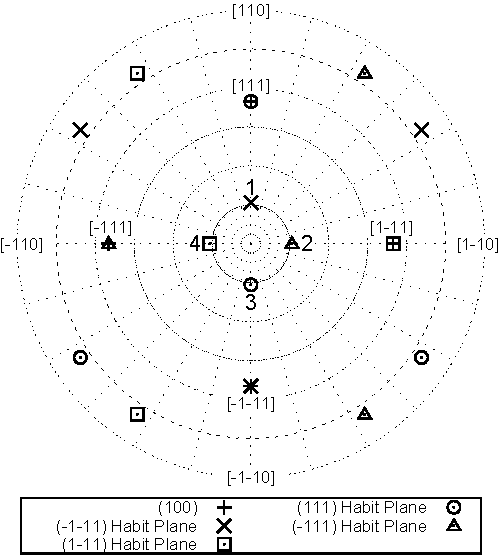
\includegraphics[width=\textwidth]{twins_sim_polefigure}
        \caption{Simulated III-V on silicon pole figure. Markers (1-4) are used to denote peaks selected
        for intensity measurements.\label{fig:twins_sim_polefigure}}
    \end{subfigure}
    \caption{\label{fig:polefigure_example}Representative pole figure and simulated pole 
    figure}
\end{figure}

Growths of III-V thin films were performed on vicinal substrates due to the established 
literature indicating the ability of atomic height steps formed by such substrates to 
overcome the polar-on-non-polar growth problem\cite{Kroemer1987}. The pole figures 
generated for thin films grown on vicinal substrates were found to have a distinctive 
asymmetry in the intensity distribution of the peaks associated with twinned orientation, 
when compared to the thin films grown on nominal silicon substrates. The pole figures for 
both nominal and vicinal substrates are shown in \cref{fig:twins_polefigure}. 
General visual differences between the pole figures across the different materials systems can be attributed to the relative diffraction intensities of the different materials.
In all cases the vicinal pole figures are oriented such that the center of symmetry is shifted away from the tilt direction, i.e. towards the atomic step edges.

\begin{figure}
    \centering
    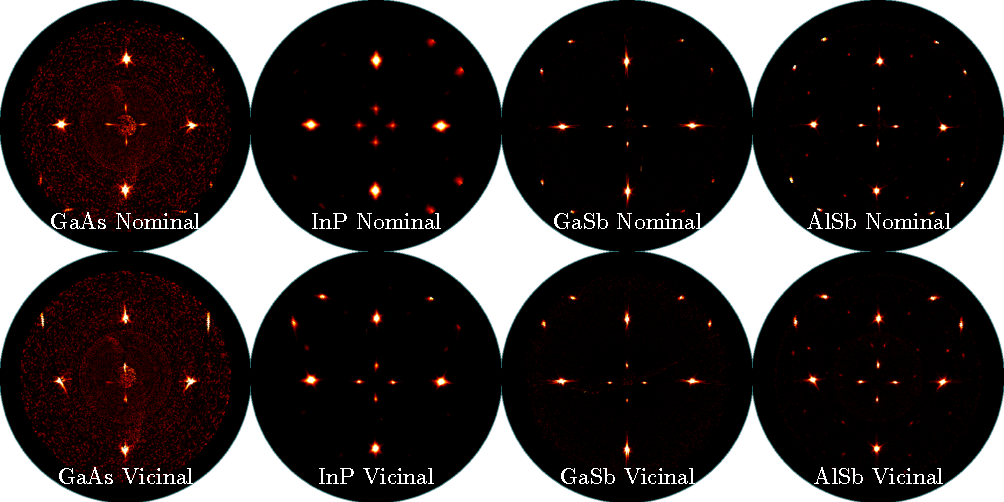
\includegraphics[width=\textwidth]{twins_polefigure}
    \caption{Stereographic \{111\} pole figures generated from 2DXRD show a bulk (100) 
    phase plus four twinned variants as identified in \cref{fig:twins_sim_polefigure}. 
    Twin variant intensity is asymmetric for vicinal 
    substrates.\label{fig:twins_polefigure}}
\end{figure}

The intensity of the peaks denoted 1-4, as labelled in \cref{fig:twins_sim_polefigure}, corresponding to a unique (111) reflection from each of the primary twins was integrated for each of the pole figures, and plotted in \cref{fig:twins_stats}.
The peak intensities were corrected for x-ray structure factor exposure time, and sample thickness where these parameters were different in order to allow comparison.
In order to better allow comparisons between material systems, in \cref{fig:twins_stats}b, intensities are normalized to the maximum for the given figure.
For thin films grown on nominal substrates, the intensity of peaks 1-4 and hence the twin volume fraction is equal within experimental uncertainty.
For all material systems, the vicinal substrates demonstrate a 50-75\% reduction in the intensity of peak 3, and hence the twin volume fraction corresponding to the twins forming opposite to the step direction.

\begin{figure}
    \centering
    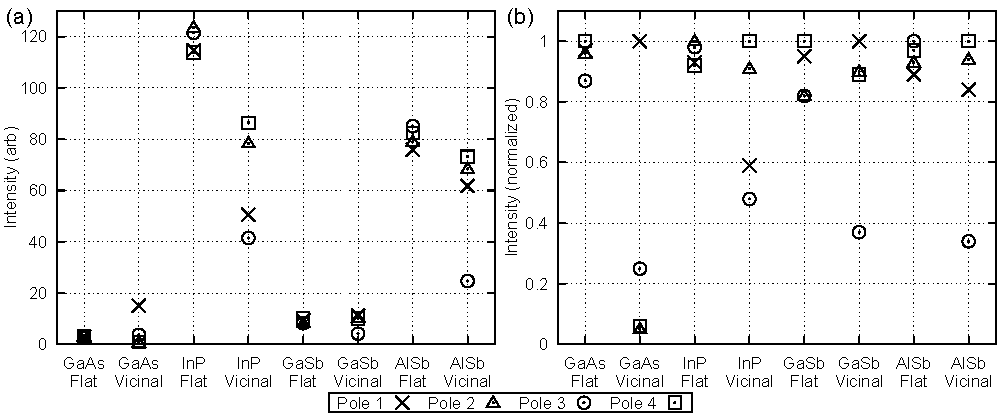
\includegraphics[width=\textwidth]{twins_stats}
    \caption{(a) Corrected (via structure factor and exposure time) and (b) normalized intensity of twin poles (as labelled in \cref{fig:twins_sim_polefigure} above). The normalized X-ray intensity clearly shows a strong reduction in Pole 3 for all vicinal substrates.\label{fig:twins_stats}}
\end{figure}

Conventional cross-sectional TEM imaging in the [1$\overline{1}$0] direction shows microtwins present in both nominal and vicinal substrate orientations as seen in \cref{fig:twins_tem}. 

\begin{figure}
    \centering
    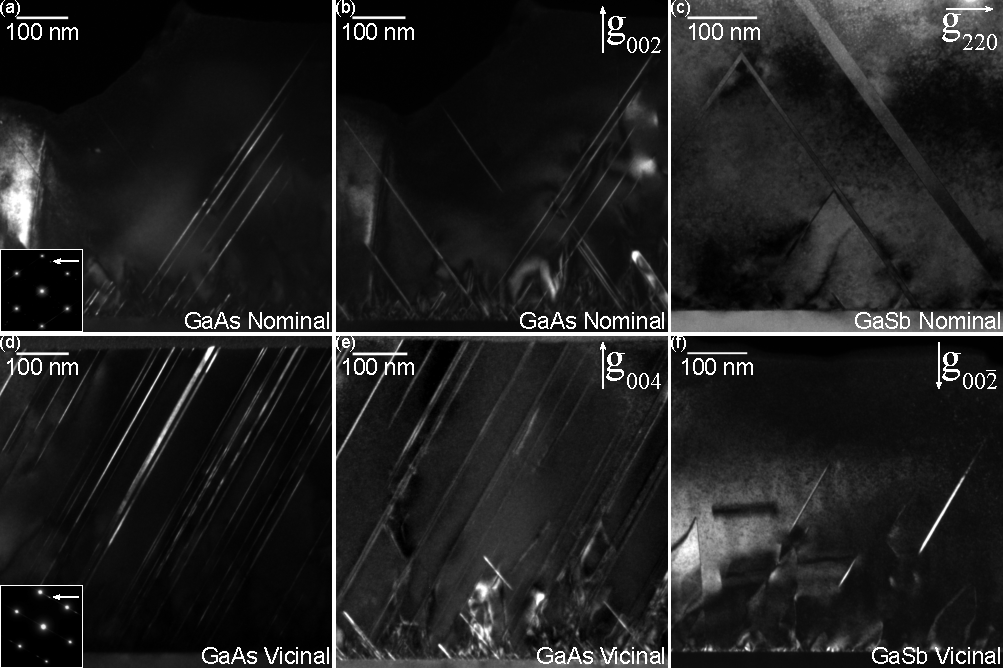
\includegraphics[width=\textwidth]{twins_tem}
    \caption{Conventional TEM images of the [1$\overline{1}$0] cross-section, (a) GaAs Nominal DF image of variants with ($\overline{1}\overline{1}$1) twin habit plane; (b) GaAs Nominal DF image of the same area as (a); (c) GaSb Nominal BF image; (d) GaAs Vicinal DF image of variants with ($\overline{1}\overline{1}$1) twin habit plane; (e) GaAs Vicinal DF image of the same area as (d); (f) GaSb Vicinal with the preferential twinning direction of ($\overline{1}\overline{1}$1) away from step edge (Pole 1), as indicated by microtwins with bright contrast in this DF image; step edge direction is towards the right for all vicinal images.\label{fig:twins_tem}}
\end{figure}